
\section{Interaction Models}

In this section, we describe how head orientation-based interaction works from the users' point of views (Figure~\ref{fig:interaction}). \sean{do we want to just use the term Glass or explains that it stands for any head-worn computing devices?}

{\bf Scan:} The user first scans the environment to locate the position of the target. During this stage, Glass constantly sends out IR signals, and the target offers immediate feedback when it receives the signal. 

{\bf Coarse Selection:} The user confirms his desire to connect to a target by tapping on the Glass touchpad. Glass collects the responses from targets regarding their IR signal reception. If there is only one single target in IR range, then it's automatically connected and the selection process is completed. However, in a relative dense environment where multiple targets are within range, the user needs to perform a fine selection.

{\bf Fine selection:} When disambiguation is needed, the user needs to make an explicit selection among the targets that within his view range. There are multiple ways to achieve it -- either from Glass touchpad that controls a GUI list or using the head motion sensor on Glass. We will provide a thorough and complete discussion later in the paper. Once the user confirms the current selection, he could tap to complete the fine selection process. Since the purpose of this stage is to effectively disambiguate among potential targets, we will also use {\em disambiguation} to refer to this stage.

\begin{figure}[t!]
\centering
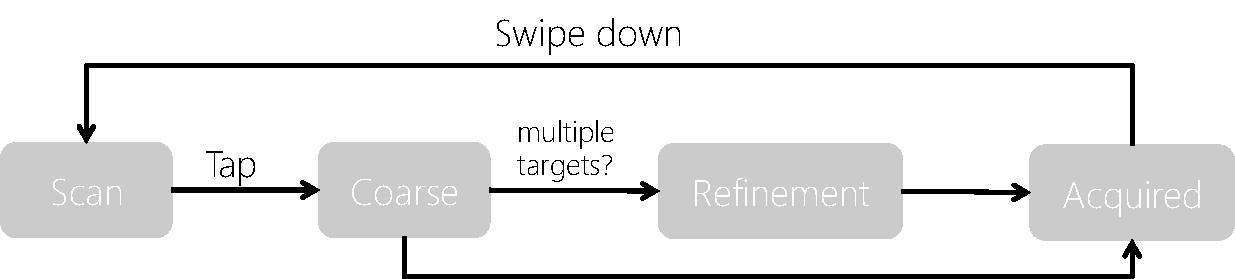
\includegraphics[width=\columnwidth]{figures/interactionModel.pdf}
\caption{Four different states during the head-orientation targeting.}
\label{fig:interaction}
\end{figure}

From the flow of interaction, we learned that the overall target acquisition time can be broken down into the following pieces:
\begin{equation}
t_{total}=t_{scan}+t_{coarse}+t_{disambiguation}
\end{equation}

Our goal of this paper is to minimize the overall target selection time. In the following few sections, we will describe our iterative design process during which we have explored the design space.

%%% Local Variables: 
%%% mode: latex
%%% TeX-master: "uist14"
%%% End: 
